\documentclass[10pt]{scrartcl}
\usepackage{xltxtra}
\usepackage[a4paper,top=2cm, bottom=2cm, left = 2.5cm, right=2cm]{geometry}
\usepackage[]{csquotes}
\usepackage[]{titlesec}
\usepackage[]{url}
\usepackage[]{paralist}
\usepackage[absolute]{textpos}
\usepackage[]{rotating}
\usepackage[]{scrpage2}
\usepackage{ctex}
\usepackage{amsmath}
\usepackage{float}
\usepackage{listings}
\pagestyle{scrheadings}
\setheadsepline[\textwidth]{0.25pt}{}
\ohead{\headmark}
\ofoot[\pagemark]{\pagemark}
\cfoot{}
\chead{}
\ihead{Xi'an Jiaotong University}
\usepackage{xcolor}
\definecolor{msdarkblue}{RGB}{54,95,145}
\definecolor{msblue}{RGB}{79,129,189}
%\titleformat{\section}[form]{layout}{labellayout}{abstand}{davorcode}[danachcode]
\titleformat{\section}[hang]{\color{msdarkblue}\Large\sffamily\bfseries}{}{0pt}{\vspace*{-6pt}}
\titleformat{\subsection}[hang]{\color{msblue}\large\sffamily\bfseries}{}{0pt}{\vspace*{-4pt}}
\titleformat{\subsubsection}[hang]{\color{msblue}\normalsize\sffamily\bfseries}{}{0pt}{}
\setsansfont[ItalicFont={Cambria Italic},BoldFont={Cambria Bold},BoldItalicFont={Cambria Bold Italic}]{Cambria}
\setmainfont[ItalicFont={Calibri Italic},BoldFont={Calibri Bold},BoldItalicFont={Calibri Bold Italic}]{Calibri}
\setmonofont[ItalicFont={Consolas Italic},BoldFont={Consolas Bold},BoldItalicFont={Consolas Bold Italic}]{Consolas}
\setlength{\parindent}{0pt}
\setlength{\parskip}{1em}
\usepackage{unicode-math}


 \lstset{ %
	language=c++,                % the language of the code
	basicstyle=\footnotesize,           % the size of the fonts that are used for the code
	numbers=left,                   % where to put the line-numbers
	numberstyle=\tiny\color{gray},  % the style that is used for the line-numbers
	stepnumber=2,                   % the step between two line-numbers. If it's 1, each line 
	% will be numbered
	numbersep=5pt,                  % how far the line-numbers are from the code
	backgroundcolor=\color{white},      % choose the background color. You must add \usepackage{color}
	showspaces=false,               % show spaces adding particular underscores
	showstringspaces=false,         % underline spaces within strings
	showtabs=false,                 % show tabs within strings adding particular underscores
	frame=single,                   % adds a frame around the code
	rulecolor=\color{black},        % if not set, the frame-color may be changed on line-breaks within not-black text (e.g. commens (green here))
	tabsize=4,                      % sets default tabsize to 2 spaces
	captionpos=b,                   % sets the caption-position to bottom
	breaklines=true,                % sets automatic line breaking
	breakatwhitespace=false,        % sets if automatic breaks should only happen at whitespace
	title=\lstname,                 % show the filename of files included with \lstinputlisting;
	% also try caption instead of title
	keywordstyle=\color{blue},          % keyword style
	commentstyle=\color{gray},       % comment style
	stringstyle=\color{mauve},         % string literal style
	escapeinside={\%*}{*)},            % if you want to add LaTeX within your code
	morekeywords={*,...}               % if you want to add more keywords to the set
}

\begin{document}
\setlength{\TPHorizModule}{1mm}
\setlength{\TPVertModule}{1mm}
\begin{titlepage}
~
\begin{textblock}{50}(-10,-10)
\begin{color}{msdarkblue}
\rule{4cm}{32cm}
\end{color}
\end{textblock}
% Logo white
\begin{textblock}{80}(50,50)
\includegraphics[height=80mm]{logo.png}\\[6pt]
{\noindent\Huge\bfseries 热流问题数值计算 }\\
{\noindent\Large\bfseries HOMEWORK \#1}
\end{textblock}
\begin{textblock}{20}(17,290)
\begin{rotate}{90}
{\huge\bfseries \textcolor{white}{能动A71 宋德培}}
\end{rotate}
\end{textblock}
\end{titlepage}
\tableofcontents
\clearpage
%\begin{abstract}
%\end{abstract}
\section{物理问题描述}
\begin{figure}[H]
	\centering
	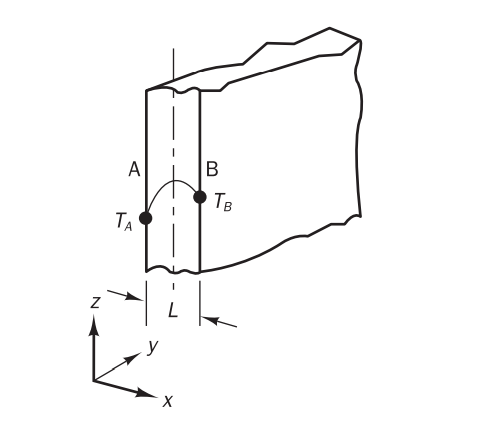
\includegraphics[width=0.4\linewidth]{1}
	\caption{问题描述}
	\label{fig:1}
\end{figure}

有一房屋的砖墙厚度为$L = 0.3\ m$,$k=0.85\ W/m\cdot^{\circ}$C,$\rho c=1.05\times 10^6 J/m^3\cdot^{\circ}$C,室内温度$T_{A}=20\ ^{\circ}$C保持不变,对流换热系数$a_1 = 6\ W/m^3\cdot ^{\circ}$C,起初墙外的温度稳定,墙内的温度分布为稳态,现在室外温度下降为$T_{B}=-10\ ^{\circ}$C,外墙表面换热系数$a_2=35\ W/m^3\cdot^{\circ}$C。则经过多长时间后内墙感受到外界温度变化。
\section{问题的数学描述}
本问题的控制方程以及边界条件、初始条件可以抽象为下述问题:
\begin{align}
	\frac{\partial T}{\partial t} = a\frac{\partial^2 T}{\partial^2 x}\\
	x=0,\ a_1(T_{A}-T) = -k\frac{\partial T}{\partial x}\\
	x=L,\ a_2(T-T_{B}) = -k\frac{\partial T}{\partial x}\\
	t=0,\ T=15-q\frac{x}{k}
\end{align}
其中$q = a_1(T_{A}-T_1)=30\ W/m^3$。
\section{离散方程建立}
程序采用均分网格计算,并且物理量储存于网格中心。
\begin{figure}[H]
	\centering
	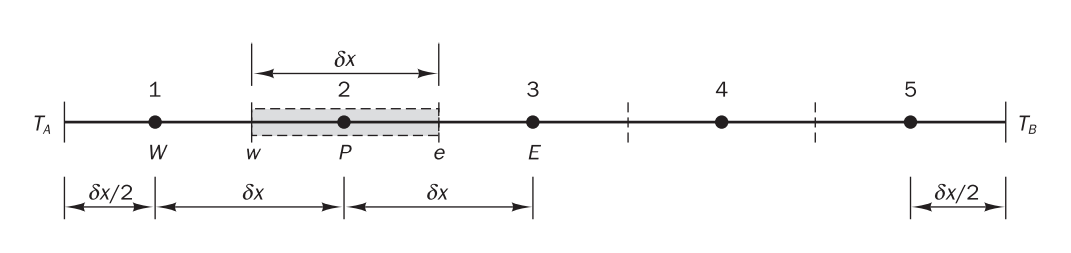
\includegraphics[width=0.8\linewidth]{2}
	\caption{均分网格示意图}
	\label{fig:2}
\end{figure}
对于无内热源的一维非稳态导热问题,控制容积内的积分方程如下:
\begin{equation}
	\int_{\Delta V}\int_{t}^{t+\Delta t}\rho c \frac{\partial T}{\partial t}dtdV=\int_{\Delta V}\int_{t}^{t+\Delta t}\frac{1}{A(x)}\frac{\partial}{\partial x}[kA(x)\frac{\partial T}{\partial x}]dtdV
\end{equation}
采用全隐格式,即取
\begin{equation}
	\int_{t}^{t+\Delta t}Tdt = T\Delta t
\end{equation}
则得到
\begin{equation}\label{res}
	\rho c \frac{T_P-{T_P}^0}{\Delta t} = k \frac{T_E-2T_P+T_W}{\Delta x^2}
\end{equation}
\subsection{稀疏矩阵系数}
对方程(\ref{res})进行整理,得到如下形式
\begin{align}
	a_PT_P = a_WT_W+a_ET_E+S_u\\
	a_P = a_W+a_E-S_p
\end{align}
由此可以获得如下的稀疏矩阵各项系数。
\begin{equation}
\left(
	\begin{array}{cccc}
	a_P^{*}& a_E^{*} &0&...  \\ 
	a_W&a_P &a_E& ... \\ 
	0& a_W & a_P&..\\
	..&...&...&...
	\end{array} 
\right)
\left(
	\begin{array}{c}
	T_1\\ 
	T_2\\ 
	T_3\\
	...
	\end{array}
\right)
=
\left(
	\begin{array}{c}
	S_u^{*}\\ 
	S_u\\ 
	S_u\\
	...
	\end{array}
\right)
\end{equation}
\begin{center}
	\begin{tabular}{|c|c|c|c|c|}
		\hline 
		$a_W$&  $a_E$&$S_p$& $S_u$ & $a_P$ \\ 
		\hline 
		$\frac{k}{\Delta x}$& $\frac{k}{\Delta x}$ &$-\rho c \frac{\Delta x}{\Delta t}$&$ \rho c \frac{\Delta x}{\Delta t}T_P^0$ &$a_w+a_E-S_p$  \\ 
		\hline 
	\end{tabular} 
\end{center}
\subsection{源项处理与附加源项法}
由于边界条件的存在,需要对边界处的离散方程做特殊处理,以下以左边界为例考虑三种边界条件,右边界的推导类似。
\subsubsection{第一类边界条件}
对边界节点的控制体积积分给出如下的守恒形式:
\begin{equation}
	k\frac{T_E-T_P}{\Delta x}-k\frac{T_P-T_A}{\Delta x/2}=\rho c \frac{T_P-{T_P}^0}{\Delta t}\Delta x
\end{equation}
因此整理可得
\begin{center}
\begin{tabular}{|c|c|c|c|c|}
	\hline 
	$a_W$&  $a_E$&$S_p$& $S_u$ & $a_P$ \\ 
	\hline 
	 0& $\frac{k}{\Delta x}$ &$-\frac{2k}{\Delta x}-\rho c \frac{\Delta x}{\Delta t}$&$ \frac{2k}{\Delta x}T_A+\rho c\frac{\Delta x}{\Delta t} T_P^0$ &$a_w+a_E-S_p$  \\ 
	\hline 
\end{tabular} 
\end{center}

\subsubsection{第二类边界条件}
第二类边界条件需要指定边界上的热流密度,假设此值在左边界为$q_A$,并且方向以进入控制体的方向为正,则可得到如下的守恒方程:
\begin{equation}
	k\frac{T_E-T_P}{\Delta x} +q_A = \rho c \frac{T_P-{T_P}^0}{\Delta t}\Delta x
\end{equation}
则整理得
\begin{center}
	\begin{tabular}{|c|c|c|c|c|}
		\hline 
		$a_W$&  $a_E$&$S_p$& $S_u$ & $a_P$ \\ 
		\hline 
		0& $\frac{k}{\Delta x}$ &$-\rho c \frac{\Delta x}{\Delta t}$&$ q_A+\rho c \frac{\Delta x}{\Delta t}T_P^0$ &$a_w+a_E-S_p$  \\ 
		\hline 
	\end{tabular} 
\end{center}
第二类边界条件中的壁面温度$T_{wall}$可以从热流密度推算出来:
\begin{equation}
	T_{wall} = T_1+\frac{q_A \Delta x}{2k}
\end{equation}

\subsubsection{第三类边界条件}
第三类边界条件相比第二类边界条件只要在守恒方程中使用$h(T_{f}-T_{wall})$代替$q_A$,其方向同样是以进入控制体为正向。使用附加源项法,从方程中去除$T_{wall}$,即使用
\begin{equation}
	q_A = \frac{T_A-T_{wall}}{\frac{1}{a_1}}=\frac{T_{wall}-T_1}{\frac{\Delta x}{2k}}=\frac{T_A-T_1}{\frac{1}{a_1}+\frac{\Delta x}{2k}}
\end{equation}
为表述简单,计$\eta = \frac{1}{\frac{1}{a_1}+\frac{\Delta x}{2k}}$,经过整理即得到:
\begin{center}
	\begin{tabular}{|c|c|c|c|c|}
		\hline 
		$a_W$&  $a_E$&$S_p$& $S_u$ & $a_P$ \\ 
		\hline 
		0& $\frac{k}{\Delta x}$ &$-\eta-\rho c \frac{\Delta x}{\Delta t}$&$ \eta T_A+\rho c \frac{\Delta x}{\Delta t}T_P^0$ &$a_w+a_E-S_p$  \\ 
		\hline 
	\end{tabular} 
\end{center}
同样,壁面温度可以从热流密度推算:
\begin{equation}
	T_{wall}=\frac{a_1T_A+\frac{2k}{\Delta x}T_1}{a_1+\frac{2k}{\Delta x}}
\end{equation}
\section{代数求解方法}

\subsection{TDMA}
\begin{lstlisting}
Vec TDMA(Vec aW, Vec aP, Vec aE, Vec Su)
{
	int size = Su.size();
	//初始化向量
	Vec P(size, 0), Q(size, 0), phi(size,0);
	//消元
	P[0] = aE[0] / aP[0];
	Q[0] = Su[0] / aP[0];
	for (int i = 1; i < size; i++)
	{
		P[i] = aE[i]/(aP[i] - aW[i]*P[i-1]);
		Q[i] = (Su[i]+aW[i]*Q[i-1])/(aP[i] - aW[i]*P[i-1]);
	}
	phi[size-1] = Q[size-1];
	//回代
	for (int i = size-1; i>0 ; i--)
		phi[i-1] = P[i-1]*phi[i]+Q[i-1];
	return phi;
}
\end{lstlisting}
TDMA算法包括消元和回代两个过程,是针对三对角矩阵最有效的直接解法,相比高斯消元法$O(n^3)$的时间复杂度,它的复杂度为$O(n)$,充分利用了矩阵稀疏性。
\subsection{Jacobi迭代}
Jacobi迭代的递推式为
\begin{equation}
	x_i^{k} =\frac{1}{a_{ii}}(b_i-\sum_{j=1,j\neq i}^{n}a_{ij}x_j^{k-1})
\end{equation}
\begin{lstlisting}
Vec jacobi(Vec aW, Vec aP, Vec aE, Vec Su, double p)
{
	int n = aW.size();
	Vec phi(n,1), phi0(n,0), errList(n,1);
	// whith origin value as 0
	while (maxabs(errList) > p)
	{
		// 迭代
		phi[0] = (aE[0]*phi0[1]+Su[0])/aP[0];
		for (int i =1; i<n-1; i++)
		{
			phi[i] = (aW[i]*phi0[i-1]+aE[i]*phi0[i+1]+Su[i])/aP[i];
		}
		phi[n-1] = (aW[n-1]*phi0[n-2]+Su[n-1])/aP[n-1];
		// 计算是否收敛
		for (int i=0; i<n; i++)
		{
			errList[i] = phi0[i] - phi[i];
			phi0[i] = phi[i];
		}
	}
	return phi;
}
\end{lstlisting}
显然迭代法耗时取决于迭代精度的选取与迭代初值,在本算例中,大致取$\epsilon = 1e-6$可保证小数点后四位的精度。
\subsection{Guass-Seidel迭代}
Guass-Seidel迭代相比Jacobi迭代利用了本步的计算结果,其递推式为
\begin{equation}
	x_i^{k} =\frac{1}{a_{ii}}(b_i-\sum_{j=1}^{i-1}a_{ij}x_j^{k}-\sum_{j=i+1}^{n}x_j^{k-1})
\end{equation}
对于三对角阵,只需要对Jacobi迭代做微小修改:
\begin{lstlisting}
	phi[i] = (aW[i]*phi[i-1]+aE[i]*phi0[i+1]+Su[i])/aP[i];
\end{lstlisting}
虽然Guass-Seidel迭代的收敛速度较快,但是由于算法利用了当前步计算的值,因此程序不容易并行化。

\subsection{多重网格技术}
\subsubsection{1.基本理论}

考虑这样的线性方程组
$$
\mathbf{A}\vec{x} = \vec{b}
$$
当使用标准迭代求解器(Gauss-Seidel,Jacobi,SOR)时,观察到收敛速度趋于“停顿”,即在几次迭代后无法有效减少误差,细化网格后,问题更加突出。 实际上,研究表明,收敛速度是误差场频率的函数,即误差从节点到节点的梯度。 如果误差以高频模式分布,则收敛速度很快。 然而,在最初的几次迭代之后,误差场被平滑(变为低频),使得收敛速度变差。

一个显而易见的想法是:既然平滑后的误差在细网格上变为了低频,那么这个误差可以在粗网格上得到有效消除,因为细网格上的低频可能是粗网格上的高频!

迭代得到的中间值设为$\vec{y}$,则
$$
\mathbf{A}\vec{y} = \vec{b} - \vec{r}
$$
$\vec{r}$为残差向量,如果用$\vec{e} = \vec{x} - \vec{y}$表示中间值和解之间的距离,则
$$
\mathbf{A}\vec{e} = \vec{r}
$$
因此这个方程与原来要解的方程具有同样的系数矩阵,如果可以解出$\vec{e}$,那么便可修正中间值。为了有效地达成这一目的,把上面的方程放到粗网格中计算,以快速光滑残差。在这之后,将$\vec{e}$再投影回细网格来修正解,如此反复迭代。

多重网格方法常用的几个名词:

 \textbf{Agglomeration} :所有的多重网格方法都需要在原始“精细”网格的基础上定义一系列粗网格。定义粗网格的过程涉及到所谓的聚集,即从原始网格中组合几个节点或控制量或系数,得到粗网格上的稀疏矩阵。
 
\textbf{Restriction}:利用插值方法将误差向量投影到粗网格上

\textbf{Prolongation}:Restriction的反过程

多重网格法的两种形式:

\textbf{Geometric multigrid}:在几何多重网格中,生成了网格的层次结构。方程在每个级别上进行离散。 几何多重网格优于代数多重网格的优点是,对于非线性问题,前者应具有更好的性能,因为系统中的非线性通过重新离散化可以降低到粗糙的水平。

\textbf{Algebraic multigrid}:该算法被称为代数多重网格方案,因为生成的粗糙层方程没有使用任何几何或在粗糙层上的重新离散。这样做的优点是不需要生成或存储粗级别的网格,也不需要在粗级别上计算通量或源项。这一特性使得AMG对于非结构化网格的使用尤为重要。

多重网格法的关键算子:

\begin{enumerate}[1)]
	\item \textbf{Prolongation算子} $\mathbf{P}$,将粗网格上的结果插值到细网格上	
	\item \textbf{Restriction算子}  $\mathbf{R}$,$\mathbf{R} = \frac{1}{2}\mathbf{P^T}$	
	\item \textbf{代数多重网格的粗网格矩阵}$ \mathbf{A_{2h}} = \mathbf{R}\mathbf{A_h}\mathbf{P}$
\end{enumerate}

\subsubsection{2.算例}

\begin{figure}[H]
	\centering
	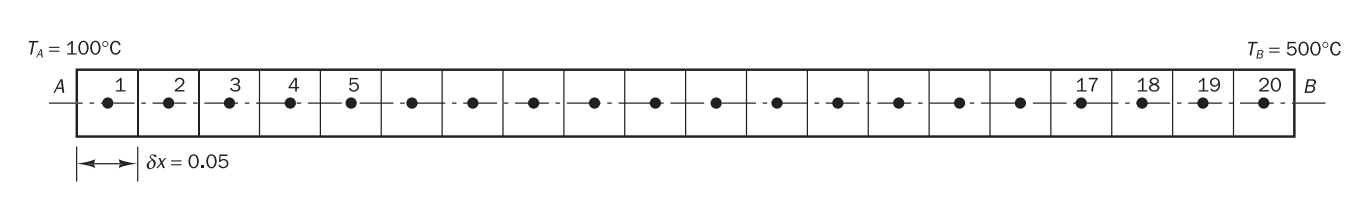
\includegraphics[width=0.7\linewidth]{multigrid}
	\caption{问题图示}
	\label{fig:multigrid}
\end{figure}


一个带内热源的导热问题
$$
k\frac{d^2T}{dx^2} + g = 0
$$
长度1m,截面积0.01$m^2$,$k = 5 W/m.K$,$q = 20 kW/m^3$

离散过程很简单,最后得到一个三对角矩阵,可以使用TDMA直接求解,在这里将使用多重网格进行求解。

\begin{enumerate}[1)]
	\item V型循环,三层网格,网格数依次为20、10、5
	\item 最后一层使用TDMA直接求解
	\item $\mathbf{P}$和$\mathbf{R}$都使用线性插值代替
	\item 粗网格矩阵可以重新离散得到或者使用插值
\end{enumerate}
\begin{lstlisting}

def restrict(vec):
	n = int(np.size(vec)/2)
	vec_coarse = np.zeros(n)
	for i in range(n):
	vec_coarse[i] = (vec[2*i]+vec[2*i+1])/2
	
	return vec_coarse


def prolong(vec):
	n = np.size(vec)
	vec_fine = np.ones(n*2)*vec[0]/2
	for i in range(1, n*2):
	if (i % 2 == 0):
	vec_fine[i] = (vec[int(i/2) - 1] + vec[int(i/2)])/2
	else:
	vec_fine[i] = vec[int(i/2)]
	
	return vec_fine


# iter stands for itereation times
def gsIter(aw, ap, ae, su, phi, itr):
	n = np.size(aw)
	phi0 = phi
	for i in range(itr):
		phi[0] = (ae[0]*phi0[1]+su[0])/ap[0]
	for i in range(n-1):
		phi[i] = (aw[i]*phi[i-1]+ae[i]*phi0[i+1]+su[i])/ap[i]
	
	phi[n-1] = (aw[n-1]*phi[n-2]+su[n-1])/ap[n-1]
	for i in range(n):
		phi0[i] = phi[i]
	
	return phi


def residual(su, aw, ap, ae, phi):
	n = np.size(su)
	res = np.zeros(n)
	for i in range(1, n-1):
		res[i] = su[i] - (-aw[i]*phi[i-1]+ap[i]*phi[i]-ae[i]*phi[i+1])
	res[0] = su[0] - ap[0]*phi[0] + ae[0]*phi[1]
	res[n-1] = su[n-1] - ap[n-1]*phi[n-1] + aw[n-1]*phi[n-2]
	return res


def getMatrix(num):
	aw = np.zeros(num)
	ap = np.zeros(num)
	ae = np.zeros(num)
	su = np.zeros(num)
	for i in range(1, num-1):
		aw[i] = k*a*num/l
		ae[i] = aw[i]
		su[i] = q*a*l/num
		ap[i] = aw[i]+ae[i]
	
	aw[0] = 0
	ae[num-1] = 0
	ae[0] = k*a*num/l
	aw[num-1] = k*a*num/l
	su[0] = q*a*l/n+2*k*a*num/l*tl
	su[num-1] = q*a*l/n+2*k*a*num/l*tr
	ap[0] = aw[0]+ae[0] + 2*k*a*num/l
	ap[num-1] = aw[num-1]+ae[num-1] + 2*k*a*num/l
	return aw, ap, ae, su


def sol(aw, ap, ae, su):
	n = np.size(aw)
	p = np.zeros(n)
	q = np.zeros(n)
	phi = np.zeros(n)
	p[0] = ae[0]/ap[0]
	q[0] = su[0]/ap[0]
	for i in range(1, n):
		p[i] = ae[i]/(ap[i] - aw[i]*p[i-1])	
		q[i] = (su[i] + aw[i]*q[i-1])/(ap[i]-aw[i]*p[i-1])
	
	phi[n-1] = q[n-1]
	for i in range(n-1, 0, -1):
		phi[i-1] = p[i-1]*phi[i]+q[i-1]

return phi

# prepare matrix
aw, ap, ae, su = getMatrix(n)
aw2, ap2, ae2, su2 = getMatrix(int(n/2))
aw3, ap3, ae3, su3 = getMatrix(int(n/4))
phi = np.ones(n)*150
phi = gsIter(aw, ap, ae, su, phi, 3)

res = 1
cnt = 0
res_list = []
while(res > 1e-6):
	# finest mesh
	phi = gsIter(aw, ap, ae, su, phi, 2)
	r = residual(su, aw, ap, ae, phi)
	res = np.mean(r)
	res_list.append(res)
	cnt += 1
	# ------------- restriction -----------------
	r2 = restrict(r)
	e2 = gsIter(aw2, ap2, ae2, r2, np.zeros(int(n/2)), 10)
	r4 = residual(r2, aw2, ap2, ae2, e2)
	rr = restrict(r4)
	#e4 = gsIter(aw3,ap3,ae3,rr,np.zeros(int(n/4)),10)
	e4 = sol(aw3, ap3, ae3, rr)
	# ------------ prolongation -----------------
	eff = prolong(e4)
	e2 = e2+eff
	e2 = gsIter(aw2, ap2, ae2, r2, e2, 2)
	ef = prolong(e2)
	phi = phi + ef

plt.figure(1)
plt.plot(res_list)
plt.show()
\end{lstlisting}


设定迭代判据为平均残差(绝对值)小于$1\times 10^{-6}$时收敛,经过27次V循环,迭代收敛。

\subsubsection{3.有效性分析}

\begin{figure}[H]
	\centering
	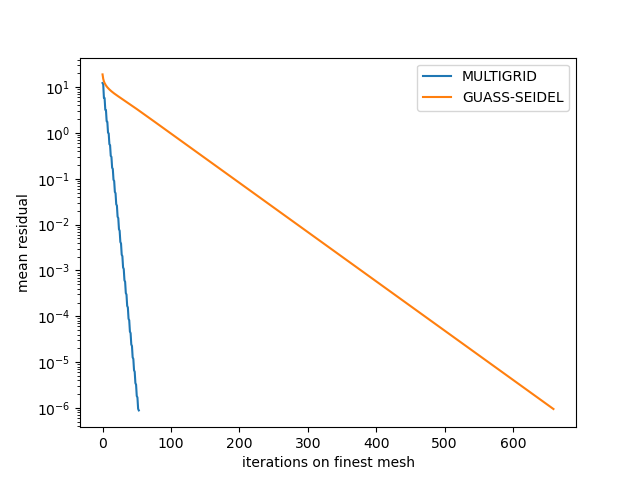
\includegraphics[width=0.6\linewidth]{result}
	\caption{迭代残差图}
	\label{fig:result}
\end{figure}


可以看到,单纯的高斯赛德尔迭代需要近660步才能迭代到收敛,而采用多重网格后,只需要27个V循环,每个循环由2次细网格上的GS迭代和10次较粗网格上的GS迭代以及最粗网格的TDMA组成,大大减少了计算量。
\section{程序框架}
此计算程序可以从控制文件读取控制参数,进行稳态或非稳态计算,可以指定三种边界条件,将温度场输出为tecplot格式,并可计算热流通量。
\subsection{Parameters类}
\begin{lstlisting}
#ifndef _PARAMETER_
#define _PARAMETER_
	
#include <vector>
#include <string>
using namespace std;
	
class Parameters
{
	private:
	public:
	int N, uS, B_L, B_R;
	double dt, L, A1, A2, RHOC, K, TA, TB, P, Q_R, Q_L;
	string solver;
	Parameters();
	~Parameters();
	int readParameters(const char *filename);
	void Coeff(vector<double> &aW, vector<double> &aP, vector<double> &aE);
	void getSource(vector<double> &Su, vector<double> &T);
	int outputFile(vector<double> vec_1, vector<double> vec_2);
};
	
#endif
\end{lstlisting}
Parameters类中readParameters和outputFiles负责从控制文件读取参数、输出计算结果,Coeff计算矩阵系数,getSource计算源项\footnote{完整代码发布至github:https://github.com/FR13ndSDP/NHT}。
\subsection{Solver}
Solver从获取的计算参数中选定代数方程组求解器,如果选择了迭代求解器,可以读取迭代精度。
\subsection{主程序}
主程序包括一个计算初始温度分布的initialize函数
\begin{lstlisting}
/*
*@description: uniform grid only for specific problem
*@variables: number of nodals: n
*@author: Fr13ndSDP
*@date: 2020-10-04 22:11:52
*/
int initialize(int N, double L, double Tw, double TA, double A1, double K, Vec &T, Vec &position)
{
	for (int i = 0; i < N; i++)
	{
		position[i] = L / (2 * N) + L / N * i;
		T[i] = Tw - A1 * (TA - Tw) / K * position[i];
	}
	return 0;
}
\end{lstlisting}

还包括一个选择结构用于决定进行稳态计算还是非稳态计算,针对特定问题的特殊输出也在主程序中编写。
\subsection{控制文件controlDict}
控制文件中各项参数及默认值如下所示。默认参数已经在Parameters类的构造函数中包含,如果未指定参数则会使用默认参数进行计算。
\begin{lstlisting}
# ------------ Geometry properties ---------------
# Geometry Length
L 0.3
# Number of nodes
N 64
# Spatial (s)
dt 60
# ------------ Physical properties ---------------
# rho*c
RHOC 1.05e6
# conductivity
K 0.85
# ------------ Initial condition -----------------
# left temperature
TA 20
# right temperature
TB -10
# ----------- Boundary condition -----------------
unSteady 1
# boudary condition
Boundary_L 3
Boundary_R 3
# heat flux if B.C 2 if choosen
Q_L 0
Q_R 0
# wall h if B.C 3 is choosen
A1 6
A2 35
# ----------- Linear solver ----------------------
# solver used: TDMA, jacobi or guassSeidel
solver TDMA
# precsion of iterative solver
P 1e-8
\end{lstlisting}

\section{问题分析}
首先绘制出随内壁面温度不断下降,直到达到稳态,整体温度场的变化情况。可以看到,当内壁面刚下降$0.1^\circ$C时,外壁面温度已经下降到了$-5^\circ$C以下,因此外壁面的冷却速率远高于内壁面。
\begin{figure}[H]
	\centering
	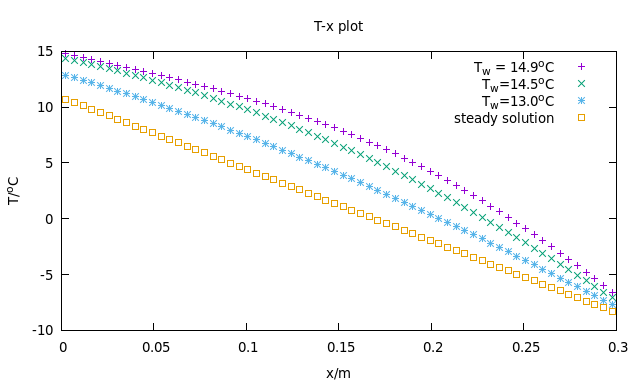
\includegraphics[width=0.7\linewidth]{multi_condition}
	\caption{温度场分布演化}
	\label{fig:multicondition}
\end{figure}
为了更加直观地了解这一现象,绘制出随时间两侧壁温的变化情况,时间轴采用对数坐标。
\begin{figure}[H]
	\centering
	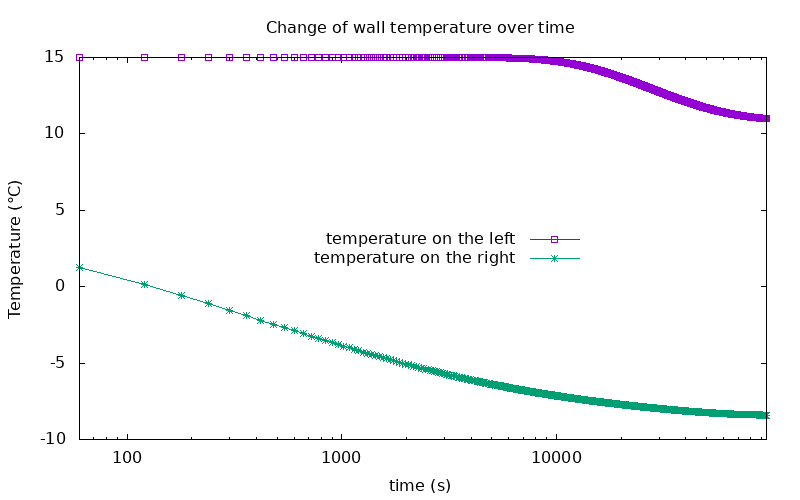
\includegraphics[width=0.7\linewidth]{t}
	\caption{两侧壁面温度变化}
	\label{fig:t}
\end{figure}
从图4中可以看出:内壁温在经过10000秒左右才发生较为强烈的降温,而外壁面的降温是从零时刻开始,这一影响是随时间逐步传递到内壁面的。

进一步地,可以绘制出两侧热流密度随时间的变化情况,分别绘制流入左壁面的热流密度与流出右壁面的热流密度。
\begin{figure}[H]
	\centering
	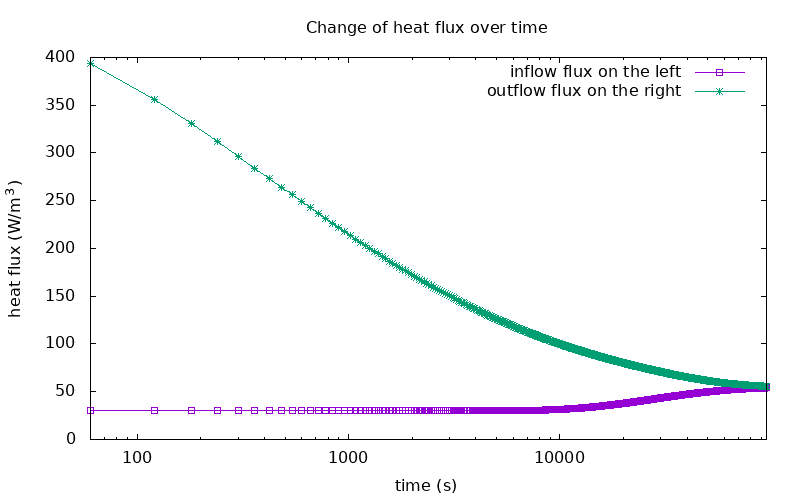
\includegraphics[width=0.7\linewidth]{flux}
	\caption{壁面热流密度变化}
	\label{fig:flux}
\end{figure}
热流密度的变化与温度变化相吻合,可以从中提取这样的一个信息:热流密度通量是温度变化的驱动力,随着右壁面流出热流密度的降低,右壁面的温度变化幅度也随之降低,而直到10000秒左右左壁面的热流密度才开始增加,此时影响传递到左壁面,温度开始下降。因此对左壁面来说,温度变化是热流密度的变化的驱动力。最终,左边界流入的热流密度与右边界流出的热流密度相等,温度场达到稳态。


\section{参考文献}
[1] 陶文铨, 数值传热学

[2] H.K.Versteeg, An introduction to computational fluid dynamics : the finite volume method

[3] J.H.Ferziger, M.Peric, Computational methods for fluid dynamics

\end{document}
